%%%%%%%%%%%%%%%%%%%%%%%%%%%%%%%%%%%%%%%%%%%%%%%%%%%%%%%%%%%%%%%%%%
% Sample template for MIT Junior Lab Student Written Summaries
% Available from http://web.mit.edu/8.13/www/Samplepaper/sample-paper.tex
%
% Last Updated August 30, 2011
%
% Adapted from the American Physical Societies REVTeK-4.1 Pages
% at http://publish.aps.org
%
% ADVICE TO STUDENTS: Each time you write a paper, start with this
%    template and save under a new filename.  If convenient, don't
%    erase unneeded lines, just comment them out.  Often, they
%    will be useful containers for information.
%
% Using pdflatex, images must be either PNG, GIF, JPEG or PDF.
%     Turn eps to pdf using epstopdf.
%%%%%%%%%%%%%%%%%%%%%%%%%%%%%%%%%%%%%%%%%%%%%%%%%%%%%%%%%%%%%%%%%%


%%%%%%%%%%%%%%%%%%%%%%%%%%%%%%%%%%%%%%%%%%%%%%%%%%%%%%%%%%%%%%%%%%
% PREAMBLE
% The preamble of a LaTeX document is the set of commands that precede
% the \begin{document} line.  It contains a \documentclass line
% to load the REVTeK-4.1 macro definitions and various \usepackage
% lines to load other macro packages.
%
% ADVICE TO STUDENTS: This preamble contains a suggested set of
%     class options to generate a ``Junior Lab'' look and feel that
%     facilitate quick review and feedback from one's peers, TA's
%     and section instructors.  Don't make substantial changes without
%     first consulting your section instructor.
%%%%%%%%%%%%%%%%%%%%%%%%%%%%%%%%%%%%%%%%%%%%%%%%%%%%%%%%%%%%%%%%%%

%\documentclass[aps,twocolumn,secnumarabic,balancelastpage,amsmath,amssymb,nofootinbib]{revtex4}
\documentclass[aps,twocolumn,secnumarabic,balancelastpage,amsmath,amssymb,nofootinbib]{revtex4-1}

%N.B. - Different computers have different packages installed.  To compile this template in the current
    % Athena environment, REVTeX 4.1 must be used.  To use the older REVTeX 4, use the commented out
    % Documentclass instead.  If you are unable to compile the template at all, you
    % may need to update your LaTeX packages.  Don't hesitate to speak with your section instructor or a 
    % TA if you're having issues getting this template to compile.

% Documentclass Options
    % aps, prl stand for American Physical Society and Physical Review Letters respectively
    % twocolumn permits two columns, of course
    % nobalancelastpage doesn't attempt to equalize the lengths of the two columns on the last page
        % as might be desired in a journal where articles follow one another closely
    % amsmath and amssymb are necessary for the subequations environment among others
    % secnumarabic identifies sections by number to aid electronic review and commentary.
    % nofootinbib forces footnotes to occur on the page where they are first referenced
        % and not in the bibliography
    % REVTeX 4.1 is a set of macro packages designed to be used with LaTeX 2e.
        % REVTeX is well-suited for preparing manuscripts for submission to APS journals.
       


\usepackage{chapterbib}    % allows a bibliography for each chapter (each labguide has it's own)
\usepackage{color}         % produces boxes or entire pages with colored backgrounds
\usepackage{graphics}      % standard graphics specifications
\usepackage[pdftex]{graphicx}      % alternative graphics specifications
\usepackage{longtable}     % helps with long table options
\usepackage{epsf}          % old package handles encapsulated post script issues
\usepackage{bm}            % special 'bold-math' package
%\usepackage{asymptote}     % For typesetting of mathematical illustrations
\usepackage{thumbpdf}
\usepackage[colorlinks=true]{hyperref}  % this package should be added after all others
                                        % use as follows: \url{http://web.mit.edu/8.13}

\renewcommand\[{\begin{equation}}
\renewcommand\]{\end{equation}}

\newcommand{\beq}{\begin{equation}}
\newcommand{\eeq}{\end{equation}}

%
% And now, begin the document...
%

\begin{document}
\title{Turning Experimental Procedures into Machine-Readable Recipes}
\author         {William Spitzer, Menghsuan Sam Pan, Iveel Tsogsuren}
\date{\today}

\begin{abstract}
Large scale manufacturing has been made more efficient with automation and machine procedures centuries ago. Scientific researches, however, still require scientists or technicians to perform the experiments due to the inherent variability and complexity. Battery research, in particular, includes large amount of hand-on experiments. In order to help automate the research, we attempt to create step-by-step machine readable procedures from experimental procedure sections of journal publications using common techniques in natural language processing. To achieve this goal, we built a pipeline process that contained several steps. First, it would take in a list of raw sentences from the experimental procedure text and label them using our custom tags to denote whether or not words were (A)ctions, (I)ngredients, (E)quipment, (PR)oducts, (P)roperties, (R)eferences, or (N)one. It would then group together words based on these labels, and separate out steps such that each step contains exactly one Action. Each step is ordered using a shift based dependency parser to connect the tagged groups with each other. Finally, it orders all of the steps based on keywords in the procedure so that each step follows chronologically from the previous step. The result is outputted as a list of dictionaries that represent each step, with details regarding what is needed to perform each step. In order to evaluate the performance of our model, we have built a small data set as our training data and development data. 
\end{abstract}

\maketitle

\section{Introduction}
The late 18th century to early 19th century marks the beginning of automation with Industrial Revolution. Since then, the ongoing advancement in technology replaces hand productions with machine manufacturing lines. Now a day, almost all the commercial products, to certain extents, are manufactured or assembled by machine production lines. In contrast, however, most of the scientific research and experiments are still done hands-on largely due to the complexity and variability these experiments can be. Therefore, the ability to convert complex human written procedures (for human) into machine readable recipes (instructions) represents one of the key barrier to fully automated research activities. Recent developments in natural language processing (NLP) researches have solved or touched upon some of the similar sub-problems in converting the instructions. For instance, identifying different contents in a experimental procedure is very similar to part of speech tagging while sorting the ingredients associated with a given action echos dependency parsing problems. 

To reduce the overall scope of this project as well as constrain the variability, this project will only deal with electrochemistry, more specifically, battery, procedures. We choose this field of study because a member of our group is extensively involved with the field. However, the model we built are meant to be generalizable to process experimental procedures in any field of study. The experimental procedures were taken from related published scientific journal such as Nano Letters, ACS Applied Materials $\&$ Interfaces, Journal of Electrochemical Society, and etc. These procedures were then processed into our training/development data by tagging with our customized experimental labels and shift-based dependency parser shifts. Then we built our NLP model using variants of well-known NLP techniques such as max-entropy classifier, shift-based dependency parser, rule based grouping algorithm, and so on. We also used widely recognized evaluation functions to determine the effectiveness of our model. 

\section{Design}

\subsection{Overall Model}

\begin{figure}
  \centering
    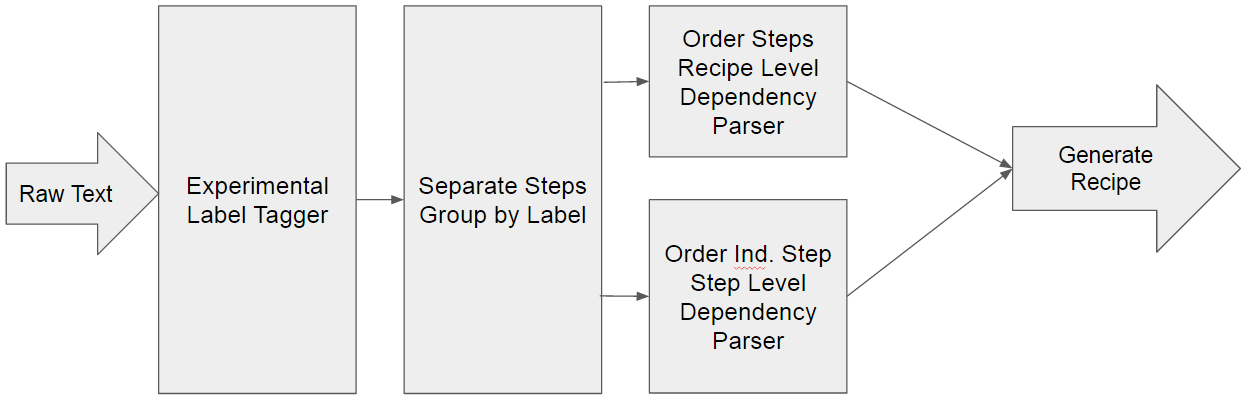
\includegraphics[width=.5\textwidth]{process.png}
  \caption{Pipeline Process. The raw text input is tagged, grouped, then ordered via dependency parsers by step level and recipe level.}
\end{figure}

Our overall goal is to take in the raw form of an experimental procedure as text and create a step by step recipe that can be performed by a machine. We defined a step as a single Action performed using some number of Ingredients, Equipments, Products, and References. Each of these can be modified by some number of Properties. We approached the problem of generating these recipes by separating the task into several tasks. The first task involves tagging individual words with a set of experimental labels (A, I, E, PR, E, R, N):  (A)ctions, (I)ngredients, (E)quipment, (PR)oducts, (P)roperties, (R)eferences, or (N)one. Following this task, we group up words from the same step together with similar labels into single entities using a rule-based system. During the grouping process, we also extract keywords that are used later to aid in determining the order of the steps such as "first", "second", "before", "after", "then" etc. Once we have the labeled entities, we want to find the relationships between different entities in each step. We applied a transition based dependency parser on these entities to determine the relationships between them. We use this information to build a tree structure that describes the steps in the experiment. 

\begin{figure}
  \centering
    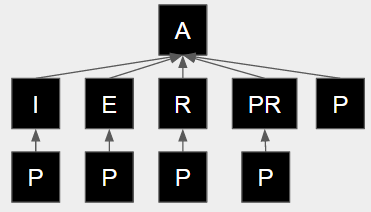
\includegraphics[width=.5\textwidth]{recipediag.png}
  \caption{Structure of a step with the Action as the root. Each action contains some number of Ingredients, Equipments, References, Products, and Properties. Each Ingredient/Equipment/Reference/Product can also be modified by additional Properties.}
\end{figure}

Finally, the steps in the experimental procedure are ordered chronologically via a second dependency parser. The output of our process is a list of dictionary structures, each corresponding to a recipe step. We provide an example of a dictionary that describes a recipe step:

\begin{figure}
  \centering
    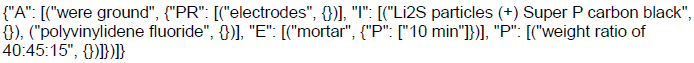
\includegraphics[width=.5\textwidth]{sampleout.png}
  \caption{Structure of a step in dictionary format.}
\end{figure}

The structure of our dictionary is as follows: The action is at the top. It contains a list of tuples of the form (“action string”, dict of modifiers). The dict of modifiers contain each possible modifier as shown in the recipe diagram below. Each modifier is again a list of tuples of the form (“modifier string”, dict of property modifiers). The dict of property modifiers is a list of properties that modify the modifier.

\subsection{Experimental Label Tagging and Move Training Set}

(A, I, E, PR, E, R, N). These tags are (A)ctions, (I)ngredients, (E)quipment, (PR)oducts, (P)roperties, (R)eferences, or (N)one. An Action is described as **TO DO** 

\subsection{Max Entropy Tagging Classifier}

\subsubsection{Description}
We built a maximum entropy tagging classifier that could tag each input word with an experimental label (EL) tag as discussed in the previous section. We took the basic structure of Honnibal's algorithm \cite{honnibal} and modified it to use additional features and our labels.

\begin{figure}
  \centering
    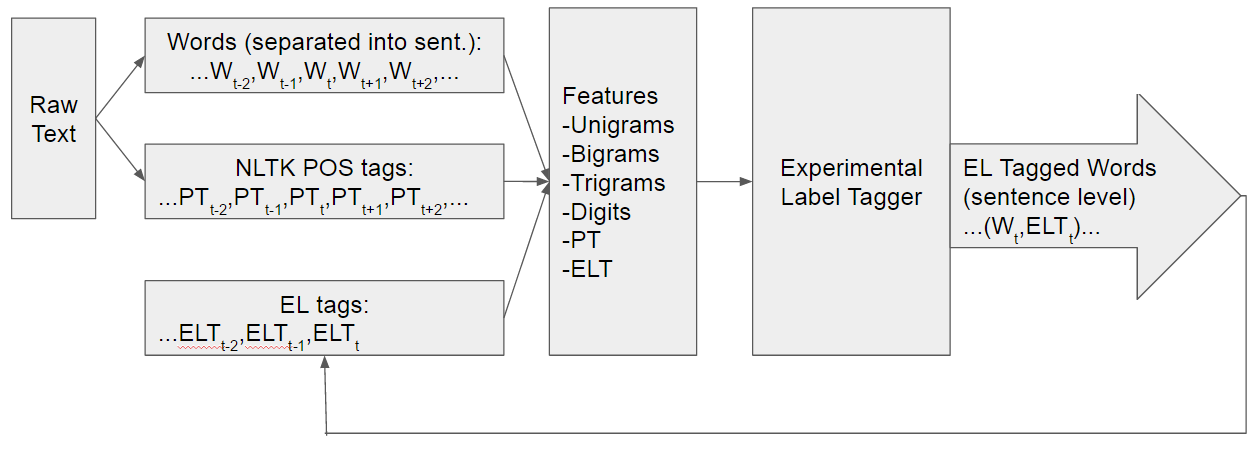
\includegraphics[width=.5\textwidth]{tagger.png}
  \caption{Structure of our Maximum Entropy Tagging Classifier.}
\end{figure}

The inputs to our classifer were lists of tokenized words from the raw text of the experiment, organized by sentence. Each alphabetical word was converted to lowercase and each numerical word was converted to a "!NUM" token. In addition, we acquired the NLTK \cite{nltk} Parts of Speech tag from the NLTK database for each word. Using the tokenized words and POS tags, we generated a wide list of features in order to best classify each word. We used the unigram, bigram, and trigram features for words, POS tags, and EL tags. We also utilized combinations of words and POS tags, and words and EL tags to capture those relationships as well. Once we have generated our features during training, we store them in a dictionary for use in evalution. The dictionary values for each feature is a list of weights corresponding to how likely a label is given that feature. Given a list of features, we can calculate an overall score for each label. Our classifier then chooses the label with the best score given the input features in order to classify each word. 

\subsubsection{Training}
Our training samples consist of experimental procedural texts that were hand annotated with our Experimental Labels. We break down the text into individual words and their labels and use those as inputs for our training. We train our classifier by creating an input feature vector for each word, allowing the classifier to perform a guess for the correct label, then updating the weights for that feature by providing the true label. Each feature that is not yet stored in our dictionary is initialized with a 1 for the correct label, and negative values for the rest, such that the sum of the weights for all labels is 0. If a feature is stored, the classifier compares the guess label with the true label. Given a positive, the weights are kept the same. Given a negative, the weight of the true label is increased by 1 and the other labels are decreased such that the overall sum of the weights for all label is still 0. 

We perform training using all the documents in our training set over several iterations (usually around 10). For each iteration, the order of the documents is shuffled to prevent possible overfitting. 

\subsubsection{Prediction}
Once we've trained our experimental label tagger, we use it for predictions. We generate the list of feature vectors for each word and apply it to our feature dictionary. If a feature exists in the dictionary, its weights are used. However, if a feature is not found, it is ignored. The final prediction is generated by summing together all the weights across all features and choosing the label with the best weight value. Our output is then lists of tagged words, where each list represents a sentence. Each word would be represented by (Raw Text, EL tag, POS tag). A sample list would look as follows:

\begin{figure}
  \centering
    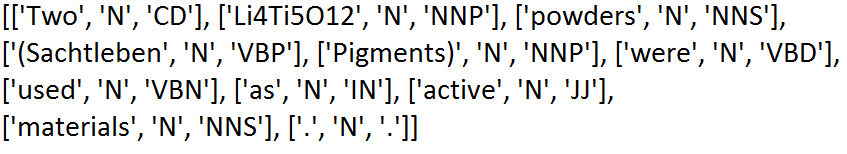
\includegraphics[width=.5\textwidth]{taggerout.png}
  \caption{Output of the EL tagging classifier.}
\end{figure}

\subsection{Grouper and Step Sorter}

We built a rule based grouping system that takes the words labeled with EL tags from the tagger and groups individual words together with similar labels, separates out steps from sentences, and extracts ordering keywords from each sentence list. The grouping system follows several main rules to combine words and create steps. Since each step should contain exactly one action, each sentence is broken so that each action in the sentence becomes its own step. The rules are as follows. First, any word that is tagged as N is ignored in grouping. Second, any uninterrupted set of words are combined together to form a phrase with the same EL tag. Third, if words with the same tag are separated by another word tagged with N, those words would also be combined. This way, we can include phrases that are separated by commas, prepositions (e.g. then, next), linking words (e.g. and, or) etc. We include a $(+)$ symbol between words combined in this way to show that they were separated initially. Fourth, if in a sentence, the grouper encounters a word with the Action tag when it has already finished tagging a previous phrase as an Action, the grouper would end construction of the current step and create a new step with the new Action tagged word as the first element. The end result of grouped steps would look as follows:

\begin{figure}
  \centering
    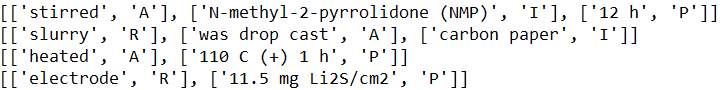
\includegraphics[width=.5\textwidth]{grouperout.png}
  \caption{Output of the grouping system.}
\end{figure}

During the grouping of each step, we also extracted keywords that would provide information in ordering the steps. These keywords include the words 'first', 'second', 'third', 'fourth', 'fifth', 'next', 'then', 'after', 'before', 'last', 'lastly', and 'finally'. The keywords in each step are stored with the step for use in the recipe level ordering. 

The output of the grouping system is two lists, where each list now represents a step in the recipe. The first is a list of phrases, each with an EL tag. The second is a list of ordering keywords, corresponding to the steps in the first list. Both lists will be used in dependency parsers in the following tasks in the pipeline process.

\subsection{Step-Level Dependency Parser}

\subsubsection{Description}
We implemented a transition based dependency parser to discover the relationships within each step between the phrases of different labels. We based the structure of our dependency parser again using Honnibal's algorithm outline.\cite{honnibal} Our dependency parser moves through the sentence one word at a time and adds arcs between the phrases. Each move is either a SHIFT, LEFT-ARC, or RIGHT-ARC. Each step finishes in $O(2n)$ time for $n$ phrases in that step. An example of the transition based dependency parser is shown:

\begin{figure}
  \centering
    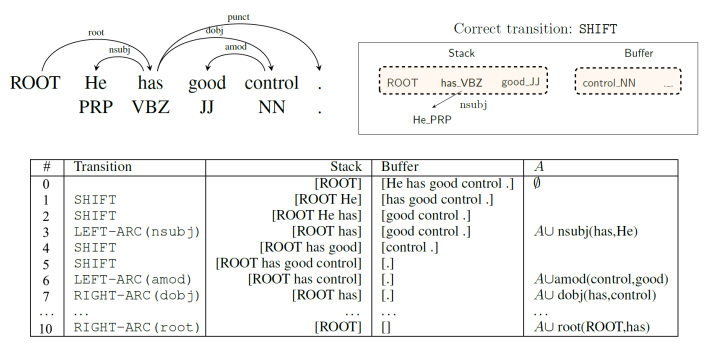
\includegraphics[width=.5\textwidth]{parser1.png}
  \caption{Demonstration of transition based dependency parser adding arcs via moves. \cite{864}}
\end{figure}

The dependency parser operates using features of the stack and buffer to determine the best move to make at any time. We build similar feature vectors as in our Tagging classifier described earlier. These features utilize the unigram, bigram, and trigram models on the phrases in the stack for both the raw text and the EL tags. We again use the weighting mechanism to determine the best move given the set of feature vectors. The features are stored within a dictionary and updated during training. Each feature has a list of 3 weights corresponding to the three possible moves (SHIFT, LEFT-ARC, RIGHT-ARC). The final move is determined by summing together all the weights from the features to find the move with the best weight. 

As the dependency parser moves through the stack and buffer, it generates a list of positions. These positions correspond to the root of the arc; the arc begins pointing to the phrase at that index in the list originated from the position value stored at that list. An example of this output corresponding to the phrases in a step is shown

\begin{figure}
  \centering
    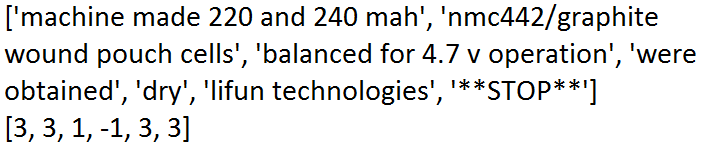
\includegraphics[width=.5\textwidth]{dep1out.png}
  \caption{Output of the step-level dependency parser. List of positions representing the arcs}
\end{figure}

\subsubsection{Training}
Our training samples consisted of hand annotated moves on the groups generated if there was perfect labeling (e.g. matched our hand-annotated labels). For each step, we would use our dependency parser to formulate a guess move and compare that move with the true move that we built. If the moves matched, we would not update the weights for the features that led to that move. However, if the moves did not match, we would update the weights by incrementing the correct move by 1 and decrementing the other two by $\frac{-1}{2}$ so that sum of all the weights of any feature still remains 0. Any feature that was not already in the dictionary of features would be initialized with a weight of 1 in the correct move and a weight of $\frac{-1}{2}$ in the other two moves. 

\subsubsection{Prediction}
For the prediction phase, the dependency parser would take in a list of labeled groups and generate a set of best scoring moves based on the feature vectors of the list of groups. The parser would then move through the list and generate a list of positions that represented the arc dependencies in that step. The final output would be a list of list of positions that represented a recipe of steps. 

\subsection{Recipe-Level Dependency Parser}

\subsubsection{Description}
The goal of this task is to order the steps in the recipe chronologically such that a machine could perform the recipe simply by going through the steps one at a time. The original experimental text may have variations in the order of the step (e.g. describe a final product first, then discuss how to generate it). We utilized the dependency parser structure that we implemented for the step-level in order to perform recipe-level dependency parsing. As such, we modified the inputs to the dependency parser, but did not change the implementation. 

These inputs are a list of order keywords generated by the grouping system that contain information about the order of the sentence. In addition, we include tags that indicate whether or not the each step contains References that match Products from the previous step. The order keyword and matching elements provide information that allows the parser to decide whether or not a step comes before or after another step. 

\subsubsection{Training}
Our training samples are hand annotated moves that denote the correct ordering of the steps in a recipe. We generated these based off of the correct list of steps of a recipe. Our dependency parser would take in these moves and train our feature dictionary weight, where the features are described in the previous dependency parser description. 

\subsubsection{Prediction}
Once trained, our dependency parser again generates a list of positions for each list of input steps that describe the ordering of the steps in terms of arcs. We construct the order using the arcs by ordering based on how the steps depend on the other steps. 

\subsection{Recipe Generation}
Once we have the outputs from both the Step-level and Recipe level dependency parsers, we can generate the entire recipe. The order of the steps is given by the list of positions from the Recipe-level dependency parser. We begin with first step in the list of positions, then move to the step that corresponds with the end of that arc. If multiple steps all originated from the same step index, we add those in order based on appearance in the list. 

To generate the recipe steps from the list of positions for each step, we perform three iterations. We first identify the location of the Action tagged group. By definition, a step contains exactly one action, so it must appear somewhere in the list. This forms the base of our step. We denote this by setting it as the first element of a tuple for the value of a dictionary containing only the key 'A'. The second element in that tuple will be a dictionary that describe the groups that are connected to the action (Ingredient/Equipment/Reference/Product/Property groups). From there, we find all the groups that have arcs connected to the action group and add them to the dictionary with keys corresponding to their label. Each group forms the first element of the tuple that describes that dictionary value. The second element is again a dictionary of Properties that describe those groups (Refer to figure 2 and 3 for visuals). Once we have generated this dictionary, we append it to the recipe list in the order prescribed by the Recipe level parser output.

Our final result is a list of dictionary representing the steps of the recipe in chronological order. 

\section{Result and Evaluation}

\section{Discussion and Future Work}

Stuff to talk about: 


The primary reason that we tag individual words and group later instead of tagging phrases as entities is due to several factors that we do not have a large number of 


\begin{thebibliography}{8}
\bibitem{honnibal}
Honnibal, Matthew. Parsing English in 500 lines of Python.
\href{https://spacy.io/blog/parsing-english-in-python}{https://spacy.io/blog/parsing-english-in-python}

\bibitem{nltk}
Natural Language Toolkit.
\href{http://www.nltk.org/}{http://www.nltk.org/}

\bibitem{864}
6.864 Lecture Notes 11. 
\href{https://learning-modules.mit.edu/service/materials/groups/105785/files/4a9be378-36a0-4dda-9e54-a29e4d8ba5b6/link}{https://learning-modules.mit.edu/service/materials/groups/105785/files/4a9be378-36a0-4dda-9e54-a29e4d8ba5b6/link}

\end{thebibliography}

\end{document}
